% Capítulo 2 - Contextualização ou definição do problema
% consiste em descrever a situação ou o contexto geral referente ao assunto em questão, devem constar informações atualizadas visando a proporcionar maior consistência ao trabalho

\chapter{Capítulo 2}

% Intonational phrase: sintagmas entoacionais
% Tone boundary: fronteira prosódica?
% Pitch accent: acento de pitch

\section{TTS}
\subsection{Breve história?}
Modelos físicos, Bell Labs, 
\subsection{Fonemas e fones}
\subsection{Abordagens}
\subsubsection{Difones}
\subsubsection{Unit selection}
\subsubsection{HMM}
\subsubsection{DNN}
Resultados realistas, mas não há como controlar parâmetros
\subsection{TTS em português}
LianeTTS (MBROLA), HMM-based (Maia et al), MaryTTS (FalaBrasil)
\section{Prosódia}
\subsection{Tipos de prosódia}
\subsubsection{Aumentativa}
\subsubsection{Suprasegmental}
\subsubsection{Afetiva}
\subsection{Elementos}
Intonational tune
Downdrift
Microprosódia
\subsection{Prosódia como elemento extra-textual}
Justifica abordagem do trabalho: considerando o texto como sequência de
palavras, é difícil determinar prosódia afetiva. Gerar a prosódia certa é uma
questão de Natural Language Understanding, isto é, é preciso entender o texto
para gerar os contornos melódicos afetivos.
\subsection{Prosódia no português brasileiro}
Trabalhos de Moraes, Tenani, ...
\subsection{Modelos de prosódia}
British school, autosegmental metrical, Fujisaki, Tilt, INTSINT
``The AM model is phonological, the INTSINT model phonetic and the Fujisaki and Tilt models acoustic.''
INTSINT: IPA para prosódia (mais ou menos o que eu quero fazer, mas INTSINT é
para análise)
ref Moraes, Intonation Systems (20 languages)
AM: Pierrehumbert, Moraes (pitch analysis by synthesis)
\subsection{Trabalhos semelhantes?}

% \begin{figure}[htb]
% 	\centering
%   	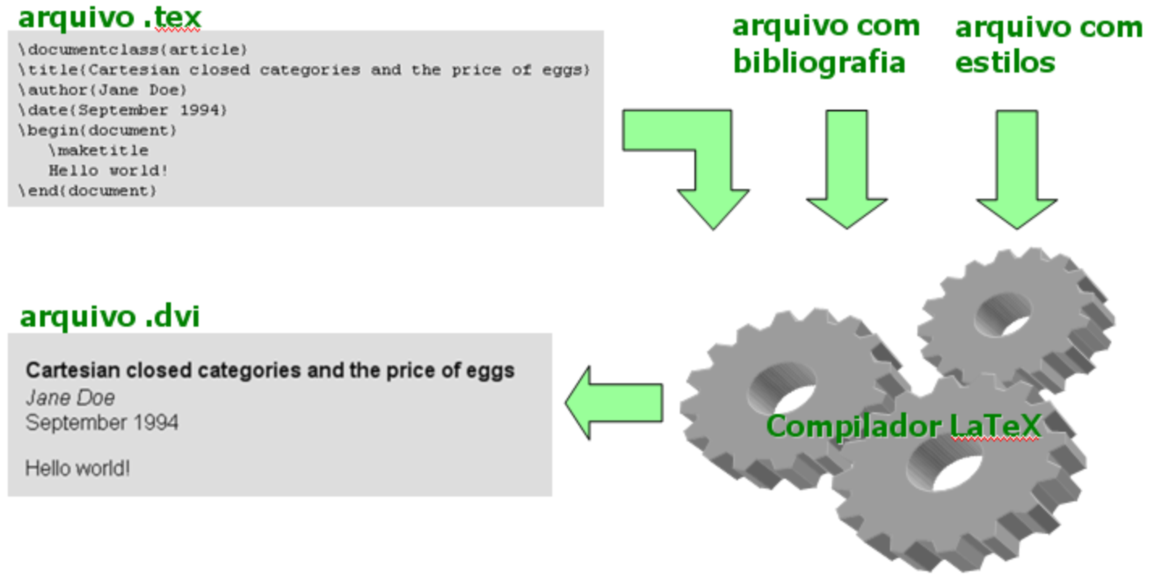
\includegraphics[scale=7.0]{Imagens/FiguraTeste.png}
%   	\textsf{\caption{Teste de uma figura em formato .png}}
%   	\label{fig:FiguraTeste}
% \end{figure}

% Referenciamento da figura inserida na seção anterior: \ref{fig:FiguraTeste}
